\subsubsection{Deep Data Analysis}

The data structure employed for analysis is depicted in Table ~\ref{tab:sales_combine_data_structure}. Following an exhaustive calculation and analysis of the initial dataset, we have arrived at a summary that provides a comprehensive overview of the findings. The results of this analysis are presented below.

\begin{table}[H]
	\centering
	\begin{tabular}{lll}
		\toprule
		& Total Sales & Total Cost \\
		\midrule
		All & \$854096.00 & \$750693.68 \\
		\bottomrule
	\end{tabular}
	\caption{Total Sales (All)}
	\label{tab:total_sales_all}
\end{table}

The total sales for all transactions is \$854,096.00, while the total cost is \$750,693.68. This results in a total sale difference of \$103,402.32.

\begin{table}[H]
	\centering
	\begin{tabular}{cccc}
		\toprule
		Day of Week & Sales & Cost & Sale Difference \\
		\midrule
		Monday & NaN & NaN & NaN \\
		Tuesday & \$166,030.00 & \$148,144.21 & \$17,885.79 \\
		Wednesday & \$169,177.00 & \$151,275.34 & \$17,901.66 \\
		Thursday & \$169,405.50 & \$151,177.94 & \$18,227.56 \\
		Friday & \$151,747.50 & \$133,614.06 & \$18,133.44 \\
		Saturday & \$107,888.50 & \$92,345.87 & \$15,542.63 \\
		Sunday & \$89,847.50 & \$74,136.26 & \$15,711.24 \\
		\bottomrule
	\end{tabular}
	\caption{Aggregated by day of week}
	\label{tab:aggregated_by_day_of_week}
\end{table}

The sales data is aggregated by day of week, showing that the highest sales are on Wednesday and Thursday, while the lowest sales are on Sunday. The cost and sale difference also vary significantly across days.

\begin{table}[H]
	\centering
	\begin{tabular}{cccc}
		\toprule
		Time Category & Sales & Cost & Sale Difference \\
		\midrule
		Breakfast & \$459,102.00 & \$409,683.85 & \$49,418.15 \\
		Lunch & \$303,747.50 & \$263,276.98 & \$40,470.52 \\
		Afternoon & \$91,246.50 & \$77,732.85 & \$13,513.65 \\
		\bottomrule
	\end{tabular}
	\caption{Aggregated by time category}
	\label{tab:aggregated_by_time_category}
\end{table}

The sales data is also aggregated by time category, showing that the highest sales are during breakfast hours, while the lowest sales are in the afternoon.

\begin{table}[H]
	\centering
	\begin{tabular}{cccc}
		\toprule
		Year & Sales & Cost & Sale Difference \\
		\midrule
		2021 & \$124,941.50 & \$109,832.82 & \$15,108.68 \\
		2022 & \$289,052.00 & \$254,140.10 & \$34,911.90 \\
		2023 & \$288,109.50 & \$253,090.72 & \$35,018.78 \\
		2024 & \$151,993.00 & \$133,630.04 & \$18,362.96 \\
		\bottomrule
	\end{tabular}
	\caption{Aggregated by year}
	\label{tab:aggregated_by_year}
\end{table}

The sales data is also aggregated by year, showing that the highest sales are in 2022 and 2023, while the lowest sales are in 2021.

\begin{figure}[H]
	\centering
	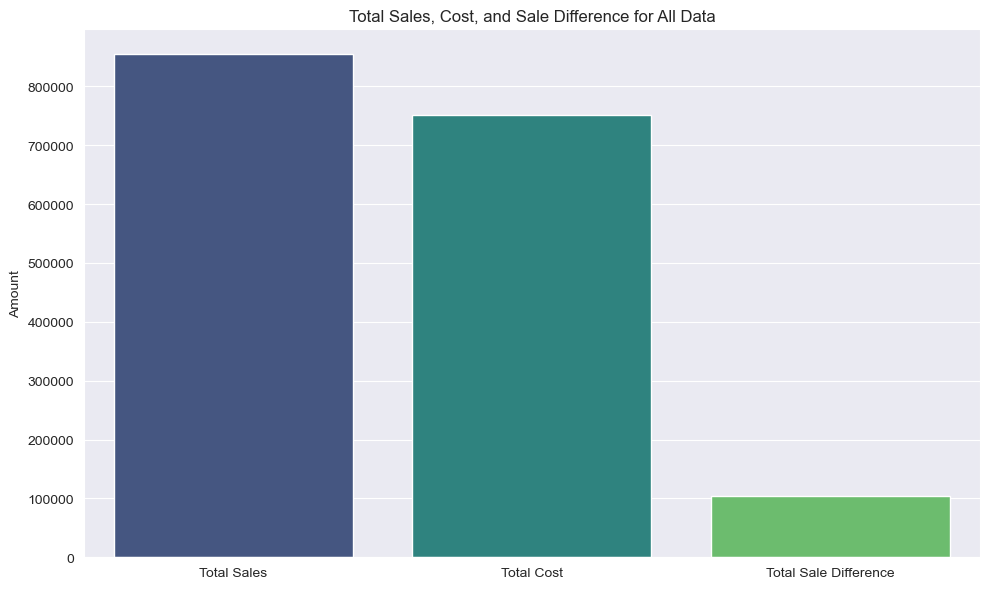
\includegraphics[width=0.8\textwidth]{assets/deep/Total Sales Cost and Sale Difference for All Data}
	\caption{Total, Sales Cost and Sale Difference for All Data}
	\label{fig:total_sales_cost_and_sale_difference_for_all_data}
\end{figure}

As illustrated by the figures above, it is evident that the cafe is not generating substantial profits, with total sales being relatively low. This suggests that the establishment requires significant increases in revenue to achieve profitability, taking into account additional expenses such as electricity bills and employer payments, which are not included in these figures.

\begin{figure}[H]
	\centering
	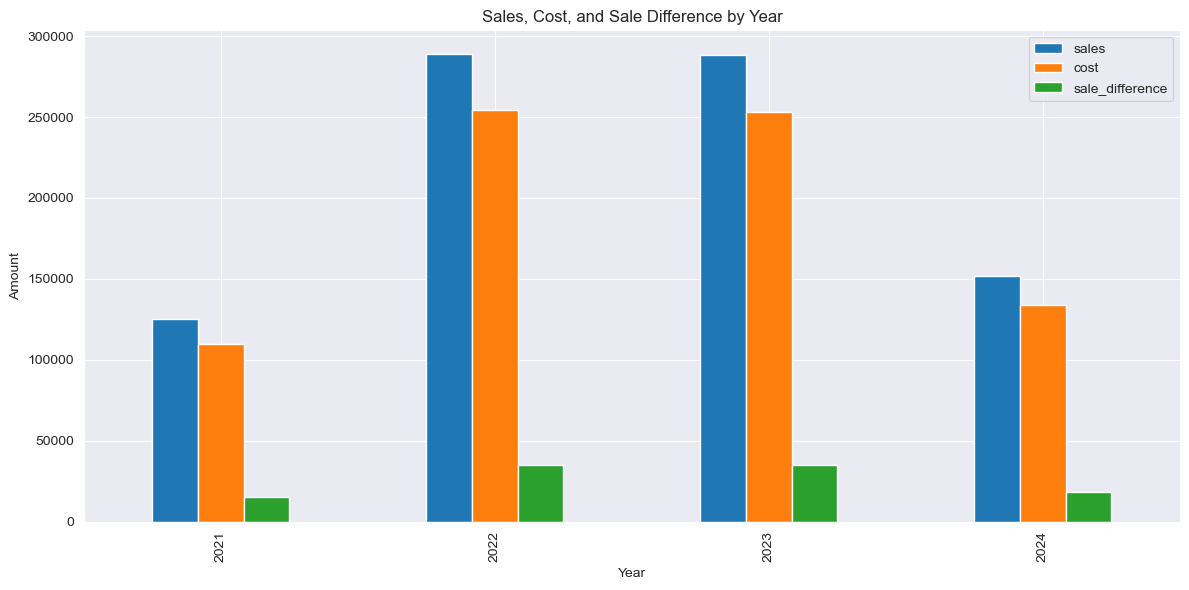
\includegraphics[width=0.8\textwidth]{assets/deep/Sales, Cost and Sale Difference by Year}
	\caption{Sales, Cost and Sale Difference by Year}
	\label{fig:sales_cost_and_sale_difference_by_year}
\end{figure}

As depicted by the figures above, it is notable that the sales amounts have remained relatively consistent across each year since 2021, with no significant fluctuations or trends observed during this period.

